\documentclass[]{article}

\usepackage{amsmath}
\usepackage{graphicx}
\usepackage{matlab-prettifier}

%opening
\title{Modeling \& Control of Boost Converter}
\author{Job Meijer}

\begin{document}

\maketitle

\begin{abstract}
\noindent Deriving the model for a boost converter, using it to simulate its behavior and derive a suitable control strategy for it.
\end{abstract}

\newpage

\section{Boost Converter Overview}
A synchronous boost converter, shown in Figure \ref{fig:boost_schematic}, consists of a voltage supply $V_{in}$, inductor $L$ with parasitic series resistance $R_{L}$, two switches in a half H-bridge configuration $S_{high}$ and $S_{low}$, a capacitor $C$ and finally the load $R$. 

\begin{figure}[h!]
	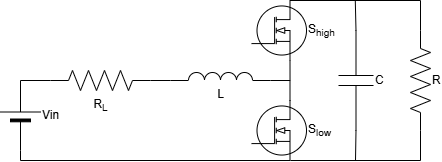
\includegraphics[scale=0.5]{images/boost_converter.png}
	\caption{Boost converter schematic.}
	\label{fig:boost_schematic}
\end{figure}

\noindent Its goal is to increase the voltage over the output load, $R$ in this case, compared to $V_{in}$. This is achieved by switching $S_{high}$ and $S_{low}$, resulting in the circuits shown in Figure \ref{fig:boost_slow} and \ref{fig:boost_shigh}. 


\begin{figure}[h!]
	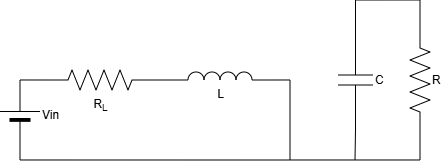
\includegraphics[scale=0.5]{images/boost_converter_slow.png}
	\caption{Boost converter schematic with $S_{low}$ switch enabled.}
	\label{fig:boost_slow}
\end{figure}

\begin{figure}[h!]
	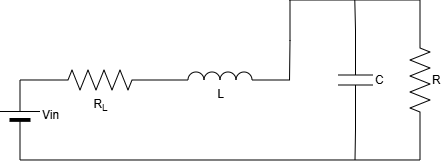
\includegraphics[scale=0.5]{images/boost_converter_shigh.png}
	\caption{Boost converter schematic with $S_{high}$ switch enabled.}
	\label{fig:boost_shigh}
\end{figure}


\newpage
\section{Deriving model}
The model is derived based on the position of the switches, resulting in two models: one with the low side switch closed, and one with the high side switch closed. \\

Starting with the low side switch closed, the Kirchhoff's circuit laws (voltage and current) are used to describe the behavior of the network: \\
\begin{equation}
	\begin{array}{l}
		v_{in}(t) - v_{R_{L}}(t) - v_{L}(t) = 0 \\
		v_{C}(t) - v_{R}(t) = 0 \\
		i_{in}(t) = i_{R_{L}}(t) = i_{L}(t) \\
		i_{C}(t) + i_{R}(t) = 0
	\end{array}
\end{equation}

Now with the high side switch closed:
\begin{equation}
	\begin{array}{l}
		v_{in}(t) - v_{R_{L}}(t) - v_{L}(t) - v_{C}(t) = 0 \\
		v_{C}(t) - v_{R}(t) = 0 \\
		i_{in}(t) = i_{R_{L}}(t) = i_{L}(t) \\
		i_{L}(t) - i_{C}(t) - i_{R}(t) = 0 
	\end{array}
\end{equation}

Next, these models are converted into a set of first order differential equations, such that it can be transformed into a state space model. \\

Quick reminder that:
\begin{equation}
	\begin{array}{l}
		v_{L}(t) = L \dfrac{di_{L}(t)}{dt} \\
		i_{C}(t) = C \dfrac{dv_{C}(t)}{dt} \\
		v_{R}(t) = i_{R}(t)R
	\end{array}
\end{equation}

Since there are two components that are able to store energy (capacitor and inductor), the minimal realization is of order 2. The variables of interest are the capacitor voltage $v_{C}(t)$ and inductor current $i_{L}(t)$. The two differential equations of interest are:
\begin{equation}
	\begin{array}{l}
		\dfrac{di_{L}(t)}{dt} = \dfrac{1}{L} v_{L}(t) \\
		\dfrac{dv_{C}(t)}{dt} = \dfrac{1}{C} i_{C}(t) \\
	\end{array}
\end{equation}

Now, for the situation with the low side switch closed, substituting
\begin{equation}
	\begin{array}{l}
		v_{L}(t) = v_{in}(t) - v_{R_{L}}(t) \\
		i_{C}(t) = i_{L}(t) - i_{R}(t) 
	\end{array}
\end{equation}

results in 
\begin{equation}
	\begin{array}{l}
		\dfrac{di_{L}(t)}{dt} = \dfrac{1}{L}(v_{in}(t) - v_{R_{L}}(t)) \\
		\dfrac{dv_{C}(t)}{dt} = \dfrac{1}{C}(i_{L}(t) - i_{R}(t)) \\
	\end{array}
\end{equation}

where $v_{R_{L}}(t) = R_{L}i_{L}(t)$, since $i_{R}(t) = i_{L}(t)$, and $i_{R}(t) = \frac{1}{R}v_{C}(t)$, since $v_{R}(t) = v_{C}(t)$, resulting in:
\begin{equation}
	\begin{array}{l}
		\dfrac{di_{L}(t)}{dt} = \dfrac{1}{L}(v_{in}(t) - R_{L}i_{L}(t)) \\
		\dfrac{dv_{C}(t)}{dt} = \dfrac{1}{C}(i_{L}(t) - \frac{1}{R} v_{C}(t)) \\
	\end{array}
\end{equation}

Furthermore, the first order differential equations for when the high side switch is closed: 
\begin{equation}
	\begin{array}{l}
		\dfrac{di_{L}(t)}{dt} = \dfrac{1}{L} v_{L}(t) \\
		\dfrac{dv_{C}(t)}{dt} = \dfrac{1}{C} i_{C}(t) \\
	\end{array}
\end{equation}

substituting 
\begin{equation}
	\begin{array}{l}
		v_{L}(t) = v_{in}(t) - v_{R_{L}}(t) - v_{C}(t) \\
		i_{C}(t) = i_{L}(t) - i_{R}(t)
	\end{array}
\end{equation}

resulting in
\begin{equation}
	\begin{array}{l}
		\dfrac{di_{L}(t)}{dt} = \dfrac{1}{L} (v_{in}(t) - v_{R_{L}}(t) - v_{C}(t)) \\
		\dfrac{dv_{C}(t)}{dt} = \dfrac{1}{C} (i_{L}(t) - i_{R}(t)) \\
	\end{array}
\end{equation}

where $v_{R_{L}}(t) = R_{L}i_{L}(t)$ and $i_{R}(t) = \frac{1}{R}v_{C}(t)$ resulting in:
\begin{equation}
	\begin{array}{l}
		\dfrac{di_{L}(t)}{dt} = \dfrac{1}{L} (v_{in}(t) - R_{L}i_{L}(t) - v_{C}(t)) \\
		\dfrac{dv_{C}(t)}{dt} = \dfrac{1}{C} (i_{L}(t) - \frac{1}{R}v_{C}(t)) \\
	\end{array}
\end{equation}

\subsection{State Space Model}
Now, the equations are transformed into a state space model, which has the form:
\begin{equation}
	\begin{array}{l}
		\dot{x}(t) = Ax(t) + Bu(t) \\
		y(t) = Cx(t) + Du(t) 
	\end{array}
\end{equation}

where $x$ is the state vector with its derivative $\dot{x}$, $u$ the input and $y$ the output vector. Defining the relations between input, state and output are the matrices $A, B, C$ and $D$. For ease of notation, the time variable $(t)$ is omitted from now on. \\

The state space model when the low side switch is on:
\begin{equation}
	\begin{array}{l}
		\begin{bmatrix}
			\frac{di_{L}}{dt} \\
			\frac{dv_{C}}{dt} \\
		\end{bmatrix}
		=
		\begin{bmatrix}
			-\frac{R_{L}}{L} & 0 \\
			0 & -\frac{1}{RC} \\	
		\end{bmatrix}
		\begin{bmatrix}
			i_{L} \\
			v_{C} \\
		\end{bmatrix}
		+
		\begin{bmatrix}
			\frac{1}{L} \\
			0 \\	
		\end{bmatrix}
		\begin{bmatrix}
			V_{in}
		\end{bmatrix} 
		\\
		\\
		\begin{bmatrix}
			V_{out}
		\end{bmatrix} 
		=
		\begin{bmatrix}
			0 & 1 \\
		\end{bmatrix}
		\begin{bmatrix}
			i_{L} \\
			v_{C} \\
		\end{bmatrix}
		+
		\begin{bmatrix}
			0 \\
		\end{bmatrix}
		\begin{bmatrix}
			V_{in} \\
		\end{bmatrix}
	\end{array}
\end{equation}

State space model when the low side is off, and high side is on:
\begin{equation}
	\begin{array}{l}
		\begin{bmatrix}
			\frac{di_{L}}{dt} \\
			\frac{dv_{C}}{dt} \\
		\end{bmatrix}
		=
		\begin{bmatrix}
			-\frac{R_{L}}{L} & -\frac{1}{L} \\
			\frac{1}{C} & -\frac{1}{RC} \\	
		\end{bmatrix}
		\begin{bmatrix}
			i_{L} \\
			v_{C} \\
		\end{bmatrix}
		+
		\begin{bmatrix}
			\frac{1}{L} \\
			0 \\	
		\end{bmatrix}
		\begin{bmatrix}
			V_{in}
		\end{bmatrix} 
		\\
		\\
		\begin{bmatrix}
			V_{out}
		\end{bmatrix} 
		=
		\begin{bmatrix}
			0 & 1 \\
		\end{bmatrix}
		\begin{bmatrix}
			i_{L} \\
			v_{C} \\
		\end{bmatrix}
		+
		\begin{bmatrix}
			0 \\
		\end{bmatrix}
		\begin{bmatrix}
			V_{in} \\
		\end{bmatrix}
	\end{array}
\end{equation}

\newpage
\section{MATLAB simulation}
To simulate the system the following MATLAB code is used:

\begin{lstlisting}[style=Matlab-editor]
%% State space model
% Mode 1: Switch ON (inductor charging)
A_on = [-R_L/L, 0; 0, -1/(R*C)];
B_on = [1/L; 0];
	
% Mode 2: Switch OFF (inductor discharging)
A_off = [-R_L/L, -1/L; 1/C, -1/(R*C)];
B_off = [1/L; 0];
	
	
%% Open loop simulation
% Simulate for N switching periods
opts = odeset('RelTol',1e-9,'AbsTol',1e-9);     % Tolerance options
[t, x] = ode45(@(t,x) boost_dyn(t,x,A_on,B_on,A_off,B_off,Vin,fsw,duty), [0 t_final], x0, opts);
	
%% Differential equation function
function dx = boost_dyn(t, x, A_on, B_on, A_off, B_off, Vin, fsw, duty)
	
	T = 1/fsw;             % Switching period
	t_mod = mod(t, T);     % Position inside switching cycle
		
	if t_mod < duty*T
		% Switch ON mode
		A = A_on;
		B = B_on;
	else
		% Switch OFF mode
		A = A_off;
		B = B_off;
	end
		
	dx = A*x + B*Vin;
end	
\end{lstlisting}

\newpage
\section{Control strategy}
Starting with the control objective.

\subsection{Objective}
Control the voltage output of the synchronous boost converter between 5 and 20V with various loads, while focussing on stability and robustness.

\subsection{Strategies}
The synchronous boost converter is a switching system. 







\end{document}
